%!TEX root = ./main.tex

\section{Experiments} \label{sec:exp}

In this section we briefly mention our empirical findings with Algorithm  1 for online linear covering problems. \cref{sec:apx-exp} gives a more in-depth analysis.

\textbf{Comparison.} The best standard online algorithm for general covering problems without experts is the online multiplicative weight update (MWU) algorithm. When a new constraint arrives in the online problem, the MWU algorithm increases each variable $x_i$ in the constraint with a rate of $\frac{a^t_i}{c_i}(x_i + 1/n)$, where $n$ is the total number of variables. We compare our algorithm with MWU algorithm.

\textbf{Input.} We evaluated the performance of Algorithm 1 on the MWU's pathological input. This instance includes $n$ variables and $n$ constraints with uniform costs and coefficients. Each arriving constraint includes one less variable. While the optimal solution is $1$, the worst-case guarantee of MWU is $O(\log n)$. For our algorithm we provided $n$ experts, where $(n-1)$ experts suggest an adversarial trivial solution to set all variables to $1$, while $1$ expert suggests the optimal offline solution. An important highlight: our algorithm managed to identify the good expert among the majority of adversaries, obtaining a better objective value, than MWU. To investigate the impact of the number of variables and the number of experts on our algorithm, we executed this example with several input sizes. The result of this experiment is visible on \cref{fig:exp-3d}.

\begin{figure}[!ht]
    \centering
    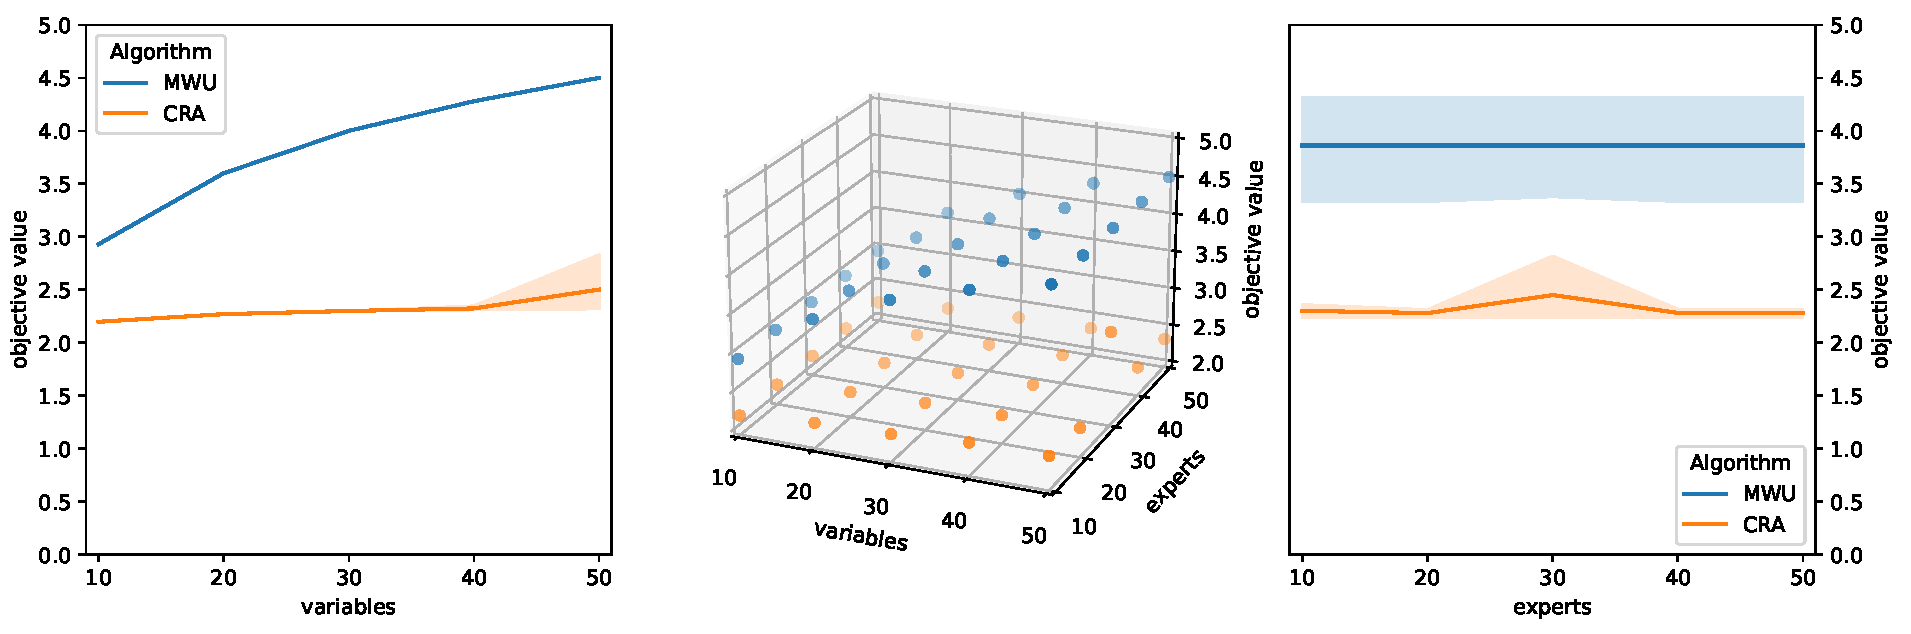
\includegraphics[width=\linewidth]{../paper/Img/worst_case_figure.pdf}
    \caption{Experiment with varying number of variables and experts on the MWU worst-case instance. The left and right plots show the result visible on the middle 3D plot with two dimensions. The shaded areas correspond to the 95\% confidence intervals.}
    \label{fig:exp-3d}
\end{figure}
